\documentclass[11pt]{article}
\usepackage[hmargin=2.2cm,vmargin=1.6cm]{geometry}
\usepackage{amsmath,amssymb,booktabs,array}
\usepackage{tikz}
\usepackage{graphicx}
\usepackage[T1]{fontenc}
\usepackage{lmodern}
\usepackage{xcolor}
\usepackage{hyperref}
\definecolor{tcol}{HTML}{E8853A}
\definecolor{ccol}{HTML}{8DB3D9}
\setlength{\parindent}{0pt}
\setlength{\parskip}{5pt}
\renewcommand{\topfraction}{0.85}\renewcommand{\bottomfraction}{0.7}\renewcommand{\textfraction}{0.1}\renewcommand{\floatpagefraction}{0.8}
\newcommand{\one}{\mathbf{1}}
\newcommand{\vzero}{\mathbf{0}}
\newcommand{\vc}{\boldsymbol{c}}
\newcommand{\vz}{\boldsymbol{z}}
\newcommand{\vb}{\boldsymbol{b}}
\newcommand{\vu}{\boldsymbol{u}}
\newcommand{\ve}{\boldsymbol{e}}
\newcommand{\vmu}{\boldsymbol{\mu}}
\newcommand{\mA}{\mathbf{A}}
\newcommand{\mM}{\mathbf{M}}
\newcommand{\mI}{\mathbf{I}}
\newcommand{\mU}{\mathbf{U}}
% \pg{fill1}{fill2}{fill3}{value under 1}{value under 2}{value under 3}
\newcommand{\pgscale}{0.85}
\newcommand{\pg}[6]{%
\begin{tikzpicture}[scale=\pgscale,transform shape,baseline=(current bounding box.center),every node/.style={circle,draw,thick,minimum size=8mm,font=\bfseries}]
\node[fill=#1] (a) at (0,0) {1};
\node[fill=#2] (b) at (1.2,1.15) {2};
\node[fill=#3] (c) at (2.4,0) {3};
\draw[thick] (a)--(b)--(c);
\if\relax\detokenize{#4#5#6}\relax\else
\node[rectangle,draw=none,minimum size=0pt,inner sep=1pt,font=\small,anchor=north,text height=1.6ex,text depth=0.4ex] at (0,-0.5) {#4};
\node[rectangle,draw=none,minimum size=0pt,inner sep=1pt,font=\small,anchor=south,text height=1.6ex,text depth=0.4ex] at (1.2,1.65) {#5};
\node[rectangle,draw=none,minimum size=0pt,inner sep=1pt,font=\small,anchor=north,text height=1.6ex,text depth=0.4ex] at (2.4,-0.5) {#6};
\fi
\end{tikzpicture}}
\usetikzlibrary{positioning}
\newcommand{\T}{\colorbox{tcol}{\strut\,T\,}}
\newcommand{\C}{\colorbox{ccol}{\strut\,C\,}}

\title{A Mathematics Tutorial on Social Network Experimentation:\\ $\rho(\mA)$, GATE, ADE and E[DM] for Linear and Log Models}
\author{M\'arton Trencs\'eni (\texttt{mtrencseni@gmail.com})}
\date{}

\begin{document}
\maketitle\vspace{-4ex}

\section*{Introduction}

Online products test changes with A/B tests: a random subset of users gets the change (treatment), the others do not (control), and the difference between the mean outcomes of the two groups estimates what launching the change to everybody would do.  This works when users do not affect each other.  On a social product they do.  A user who posts more gives the friends more content to see, and the friends may post more in response, which their friends see, and so on.  Treated users then raise the outcomes of control users, and the difference between the two groups no longer measures the effect of a launch.  This is called interference \cite{hudgens2008}; its effect on A/B tests on networks, and designs that reduce it, such as randomizing clusters of friends instead of single users, are studied in \cite{ugander2013,aronow2017,eckles2017,savje2021}.

This note uses the simplest model of such peer effects: each user's posting rate is a baseline, plus the treatment effect if treated, plus a fraction $\nu$ of what the friends post.  This is the linear-in-sums (local-aggregate) model of peer effects \cite{ballester2006}, in which a user responds to the sum of what the friends post; in the linear-in-means model studied in \cite{manski1993,bramoulle2009} a user responds to the average instead.  The steady state of the sum model is a Katz-Bonacich centrality of the friendship graph \cite{katz1953,bonacich1987}.  In this model every quantity of interest is a closed-form expression of one matrix, $\mM = (\mI - \nu\mA)^{-1}$, where $\mA$ is the friendship graph.  The note computes all of them by hand on the smallest graph that has a hub: three users on a path, $1 - 2 - 3$, where user 2 is friends with both others.  Sections 1 to 3 set up the model, its steady state $\vc(\vz) = \mM(\lambda\one + \Delta\lambda\vz)$ and the stability condition $\nu\rho(\mA) < 1$, where $\rho(\mA)$ is the spectral radius of the graph; Sections 4 to 6 compute the launch effect (GATE), the average direct effect (ADE) and what an A/B test reports (DM and E[DM]); Section 7 replaces the linear response by a logarithmic one, which has to be solved numerically.
The example shows the main point: on average the A/B test reports something close to the ADE (on a large graph whose multiplier GATE$/$ADE is much smaller than the number of users, almost exactly the ADE), while the launch effect is the GATE, and the gap between them is the spillover between friends.  All values are exact fractions; decimals are rounded.  The companion paper \emph{Network Effects in Randomized Experiments: Simulations at Scale} uses these formulas on five families of random graphs with up to $10^9$ users.

Notation: bold lowercase letters are column vectors ($\vc(\vz)$, $\vz$, $\one$), bold uppercase letters are matrices ($\mA$, $\mM$, $\mI$), and plain italic letters are scalars, including the entries of vectors and matrices ($c_i$, $A_{ij}$, $M_{ij}$).

Parameters: baseline posting $\lambda = 1$, treatment effect $\Delta\lambda = 0.1$, peer effect $\nu = 1/4$.

\section{The graph and the model}

\begin{center}
\pg{white}{white}{white}{}{}{}
\qquad
$\mA = \begin{pmatrix} 0 & 1 & 0 \\ 1 & 0 & 1 \\ 0 & 1 & 0 \end{pmatrix}$
\end{center}

$A_{ij} = 1$ if users $i$ and $j$ are friends.  Each user posts $\lambda$, plus $\Delta\lambda$ if treated ($z_i = 1$), plus $\nu$ times what the friends post:
\[
c_i(\vz) = \lambda + \Delta\lambda z_i + \nu \sum_j A_{ij} c_j(\vz) ,
\qquad\text{in matrix form}\qquad
\vc(\vz) = \lambda\one + \Delta\lambda \vz + \nu \mA \vc(\vz) .
\]
Here $\vc(\vz)$, $\one$ and $\vz$ are column vectors with one entry per user; we write $\vc(\vz)$ because the posting depends on who is treated.  $\lambda$, $\Delta\lambda$ and $\nu$ are scalars, and $z_i \in \{0, 1\}$ marks treated users.  Written out for the three users:
\[
\underbrace{\begin{pmatrix} c_1 \\ c_2 \\ c_3 \end{pmatrix}}_{\vc(\vz)}
=
\lambda \underbrace{\begin{pmatrix} 1 \\ 1 \\ 1 \end{pmatrix}}_{\one}
{}+ \Delta\lambda \underbrace{\begin{pmatrix} z_1 \\ z_2 \\ z_3 \end{pmatrix}}_{\vz}
{}+ \nu \underbrace{\begin{pmatrix} 0 & 1 & 0 \\ 1 & 0 & 1 \\ 0 & 1 & 0 \end{pmatrix}}_{\mA}
\underbrace{\begin{pmatrix} c_1 \\ c_2 \\ c_3 \end{pmatrix}}_{\vc(\vz)}
=
\begin{pmatrix} \lambda + \Delta\lambda z_1 + \nu c_2 \\ \lambda + \Delta\lambda z_2 + \nu (c_1 + c_3) \\ \lambda + \Delta\lambda z_3 + \nu c_2 \end{pmatrix}.
\]
Row $i$ of $\mA \vc(\vz)$ is the sum of the friends' posting: user 2 sees users 1 and 3, the end users see only user 2.

Example: user 1 treated, $\vz = \ve_1 = (1, 0, 0)^\top$, with $\lambda = 1$, $\Delta\lambda = 0.1$, $\nu = 1/4$.  The steady state (computed in Section 5) is $\vc(\ve_1) = (43/28,\ 61/35,\ 201/140) = (1.5357,\ 1.7429,\ 1.4357)$, and it satisfies the equation:
\[
\begin{pmatrix} 1.5357 \\ 1.7429 \\ 1.4357 \end{pmatrix}
=
1 \begin{pmatrix} 1 \\ 1 \\ 1 \end{pmatrix}
+ 0.1 \begin{pmatrix} 1 \\ 0 \\ 0 \end{pmatrix}
+ \frac14 \begin{pmatrix} 0 & 1 & 0 \\ 1 & 0 & 1 \\ 0 & 1 & 0 \end{pmatrix}
\begin{pmatrix} 1.5357 \\ 1.7429 \\ 1.4357 \end{pmatrix}
=
\begin{pmatrix} 1 + 0.1 + \frac14 \cdot 1.7429 \\[2pt] 1 + 0 + \frac14 (1.5357 + 1.4357) \\[2pt] 1 + 0 + \frac14 \cdot 1.7429 \end{pmatrix}
=
\begin{pmatrix} 1.5357 \\ 1.7429 \\ 1.4357 \end{pmatrix}.
\]

\section{The steady state $\vc(\vz) = \mM(\lambda\one + \Delta\lambda \vz)$ with $\mM = (\mI - \nu \mA)^{-1}$}

Write $\vb = \lambda\one + \Delta\lambda \vz$.  At the steady state $\vc(\vz)$ appears on both sides; solve for it:
\[
\vc(\vz) - \nu \mA \vc(\vz) = \vb
\;\Longrightarrow\;
(\mI - \nu \mA)\, \vc(\vz) = \vb
\;\Longrightarrow\;
\vc(\vz) = (\mI - \nu \mA)^{-1} \vb = \mM \vb .
\]
For this graph:
\[
\mI - \nu \mA = \begin{pmatrix} 1 & -\tfrac14 & 0 \\ -\tfrac14 & 1 & -\tfrac14 \\ 0 & -\tfrac14 & 1 \end{pmatrix},
\qquad
\det(\mI - \nu \mA) = 1\cdot\left(1 - \tfrac1{16}\right) - \tfrac14\cdot\tfrac14 = \tfrac78 ,
\]
\[
\mM = (\mI - \nu \mA)^{-1} =
\begin{pmatrix} \tfrac{15}{14} & \tfrac27 & \tfrac1{14} \\[2pt] \tfrac27 & \tfrac87 & \tfrac27 \\[2pt] \tfrac1{14} & \tfrac27 & \tfrac{15}{14} \end{pmatrix}
=
\begin{pmatrix} 1.071 & 0.286 & 0.071 \\ 0.286 & 1.143 & 0.286 \\ 0.071 & 0.286 & 1.071 \end{pmatrix}.
\]
$M_{ij}$ is how much user $i$'s posting rises per unit of posting added at user $j$, after all feedback has settled.  $M_{31} = 1/14$ is positive although users 1 and 3 are not friends: the effect passes through user 2.

\subsection{Where $\mM$ comes from: the iteration and walks}

Start from $\vc_0 = \vzero$ and repeat $\vc_{t+1} = \vb + \nu \mA \vc_t$.  Then
\[
\vc_t = \left(\mI + \nu \mA + \nu^2 \mA^2 + \dots + \nu^{t-1} \mA^{t-1}\right) \vb ,
\qquad\text{so, if it converges,}\qquad
\mM = \sum_{k \ge 0} (\nu \mA)^k .
\]
$(\mA^k)_{ij}$ counts the walks of length $k$ from $i$ to $j$:
\[
\mA^2 = \begin{pmatrix} 1 & 0 & 1 \\ 0 & 2 & 0 \\ 1 & 0 & 1 \end{pmatrix},\quad
\mA^3 = \begin{pmatrix} 0 & 2 & 0 \\ 2 & 0 & 2 \\ 0 & 2 & 0 \end{pmatrix},\quad
\mA^4 = \begin{pmatrix} 2 & 0 & 2 \\ 0 & 4 & 0 \\ 2 & 0 & 2 \end{pmatrix}.
\]
Check one entry: $M_{11} = 1 + \nu^2\cdot 1 + \nu^4 \cdot 2 + \nu^6 \cdot 4 + \dots = 1 + \tfrac12 \sum_{k\ge1} (2\nu^2)^k = 1 + \tfrac12\cdot\tfrac{1/8}{7/8} = \tfrac{15}{14}$, as in the inverse.

The iteration with $\vb = \one$ (nobody treated) reaches $\mM\one$:

\begin{center}
\begin{tabular}{rccc}
\toprule
$t$ & user 1 & user 2 & user 3 \\
\midrule
1 & 1 & 1 & 1 \\
2 & 1.25 & 1.5 & 1.25 \\
3 & 1.375 & 1.625 & 1.375 \\
5 & 1.422 & 1.703 & 1.422 \\
10 & 1.429 & 1.714 & 1.429 \\
\midrule
$\mM\one$ & $10/7 = 1.4286$ & $12/7 = 1.7143$ & $10/7 = 1.4286$ \\
\bottomrule
\end{tabular}
\end{center}

\section{The spectral radius and the stability condition $\nu\rho(\mA) < 1$}

The eigenvalues of $\mA$ solve
\[
\det(\mA - \mu \mI) = -\mu^3 + 2\mu = 0
\quad\Longrightarrow\quad
\mu \in \{-\sqrt2,\; 0,\; +\sqrt2\} .
\]
The spectral radius $\rho(\mA)$ is the largest absolute eigenvalue of $\mA$: $\rho(\mA) = \sqrt2 \approx 1.414$, with eigenvector $\vu = (1, \sqrt2, 1)/2$, largest at the hub.  The mean degree is $\bar k = 4/3$; $\rho$ is larger because the hub's two friends count for more than the average suggests.

\textbf{Why the iteration converges when $\nu\rho < 1$.}  $\mA$ is symmetric, so it has real eigenvalues $\mu_i$ and orthonormal eigenvectors $\vu_i$ ($\vu_i^\top \vu_i = 1$, $\vu_i^\top \vu_j = 0$ for $i \ne j$), and it can be written as a product of three matrices: the eigenvectors as the columns of $\mU$, the eigenvalues on the diagonal, and $\mU^\top$.  For this graph:
\[
\mA = \mU \,\mathrm{diag}(\vmu)\, \mU^\top
=
\begin{pmatrix} \tfrac12 & \tfrac1{\sqrt2} & \tfrac12 \\[2pt] \tfrac{\sqrt2}{2} & 0 & -\tfrac{\sqrt2}{2} \\[2pt] \tfrac12 & -\tfrac1{\sqrt2} & \tfrac12 \end{pmatrix}
\begin{pmatrix} \sqrt2 & 0 & 0 \\ 0 & 0 & 0 \\ 0 & 0 & -\sqrt2 \end{pmatrix}
\begin{pmatrix} \tfrac12 & \tfrac{\sqrt2}{2} & \tfrac12 \\[2pt] \tfrac1{\sqrt2} & 0 & -\tfrac1{\sqrt2} \\[2pt] \tfrac12 & -\tfrac{\sqrt2}{2} & \tfrac12 \end{pmatrix},
\]
with $\vu_1 = (1, \sqrt2, 1)/2$ for $\mu_1 = \sqrt2$, $\vu_2 = (1, 0, -1)/\sqrt2$ for $\mu_2 = 0$ and $\vu_3 = (1, -\sqrt2, 1)/2$ for $\mu_3 = -\sqrt2$.  (Check: $\mA \vu_3 = (-\sqrt2, 2, -\sqrt2)/2 = -\sqrt2\, \vu_3$.)  Multiplying out the product gives the same thing as a sum of one matrix per eigenvalue, $\mA = \sum_i \mu_i \vu_i \vu_i^\top$.

Powers are easy in this form, because $\mU^\top \mU = \mI$ cancels between neighboring factors:
\[
\mA^k = \mU \,\mathrm{diag}(\vmu)\, \underbrace{\mU^\top \mU}_{\mI} \,\mathrm{diag}(\vmu)\, \mU^\top \cdots = \mU \,\mathrm{diag}(\mu_1^k, \mu_2^k, \mu_3^k)\, \mU^\top ,
\qquad
(\nu \mA)^k \vb = \sum_i (\nu\mu_i)^k\, (\vu_i^\top \vb)\, \vu_i .
\]
So the part of $\vb$ along $\vu_i$, which is $(\vu_i^\top \vb)\, \vu_i$, is multiplied by $(\nu\mu_i)^k$ at step $k$.  The sum $\sum_k (\nu \mA)^k \vb$ converges exactly when $|\nu\mu_i| < 1$ for every $i$, that is, when $\nu\rho(\mA) < 1$, because $\rho(\mA) = \max_i |\mu_i|$ is the largest eigenvalue in absolute value.  The absolute value matters: here $\mu_3 = -\sqrt2$ is as large as $\mu_1 = \sqrt2$, and its part of $\vb$ would alternate in sign and grow if $\nu\sqrt2 \ge 1$.  Here $\nu\rho = \sqrt2/4 \approx 0.354$.

\textbf{Why the steady state is nonnegative.}  Every term $(\nu \mA)^k \vb$ has nonnegative entries, since $\mA$, $\vb$ and $\nu$ are nonnegative; so does the sum.

\textbf{Why it fails when $\nu\rho \ge 1$.}  The eigenvector $\vu$ of $\rho$ is positive (Perron-Frobenius theorem \cite[Ch.~8]{horn2013}), and $\vb = \lambda\one$ is positive, so $\vb$ has a positive part along $\vu$.  That part is multiplied by $(\nu\rho)^k \ge 1$ at every step, and the sum diverges.  With $\nu = 0.8$, $\nu\rho = 1.13$:

\begin{center}
\begin{tabular}{rccc}
\toprule
$t$ & user 1 & user 2 & user 3 \\
\midrule
2 & 1.8 & 2.6 & 1.8 \\
10 & 15.7 & 22.6 & 15.7 \\
20 & 69.5 & 100.3 & 69.5 \\
60 & 10\,572 & 15\,270 & 10\,572 \\
\bottomrule
\end{tabular}
\end{center}

The values grow by about 1.13 per step.  The inverse still exists, $\det(\mI - 0.8\mA) = 1 - 2\cdot 0.8^2 = -0.28 \ne 0$, but
\[
(\mI - 0.8\mA)^{-1} = \begin{pmatrix} -1.29 & -2.86 & -2.29 \\ -2.86 & -3.57 & -2.86 \\ -2.29 & -2.86 & -1.29 \end{pmatrix},
\qquad
(\mI - 0.8\mA)^{-1}\one = (-6.43,\, -9.29,\, -6.43),
\]
a negative posting rate that the process never reaches.  Hence the condition: the iteration converges if and only if $\nu\rho(\mA) < 1$, and only then is the solution of $(\mI - \nu\mA)\vc = \vb$ nonnegative, that is, a posting rate the process can reach.

\section{GATE $= \Delta\lambda\, \one^\top \mM \one / N$}

The global average treatment effect compares two worlds: everybody treated and nobody treated.  In the drawings, treated users are \T{} and control users are \C.  Recall the steady state from Section 2:
\[
\vc(\vz) = \mM(\lambda\one + \Delta\lambda \vz), \qquad \mM = (\mI - \nu\mA)^{-1}.
\]
Remember: $\vc(\vz)$ is the vector of how much each user posts at the steady state, and $\vz$ is the vector of treatment assignments, $z_i = 1$ if user $i$ is treated and $z_i = 0$ if not.  Nobody treated is $\vz = \vzero$, everybody treated is $\vz = \one$:

\begin{center}
\begin{tabular}{c@{\qquad}c}
\pg{ccol}{ccol}{ccol}{$10/7$}{$12/7$}{$10/7$} &
\pg{tcol}{tcol}{tcol}{$11/7$}{$66/35$}{$11/7$} \\ \noalign{\vspace{9pt}}
$\vz = \vzero$: \;$\vc(\vzero) = \mM\lambda\one$ & $\vz = \one$: \;$\vc(\one) = \mM(\lambda + \Delta\lambda)\one$
\end{tabular}
\end{center}

Subtracting,
\[
\vc(\one) - \vc(\vzero) = \Delta\lambda\, \mM \one .
\]
This vector holds each user's change in posting between the two worlds.  The GATE is its average over the $N$ users: sum the entries (multiply by $\one^\top$ from the left) and divide by $N$,
\[
\text{GATE} = \frac{1}{N}\sum_i \bigl(c_i(\one) - c_i(\vzero)\bigr) = \frac{\one^\top\bigl(\vc(\one) - \vc(\vzero)\bigr)}{N} = \Delta\lambda\,\frac{\one^\top \mM \one}{N} .
\]
$\one^\top \mM \one$ is the sum of all entries of $\mM$.  In words: the GATE is how many extra posts per user, on average, we would see if we rolled out the treatment to everybody.  The numbers:

\begin{center}
\begin{tabular}{lccc}
\toprule
 & user 1 & user 2 & user 3 \\
\midrule
$\vc(\vzero)$ & $10/7 = 1.4286$ & $12/7 = 1.7143$ & $10/7 = 1.4286$ \\
$\vc(\one)$ & $11/7 = 1.5714$ & $66/35 = 1.8857$ & $11/7 = 1.5714$ \\
difference & $1/7 = 0.1429$ & $6/35 = 0.1714$ & $1/7 = 0.1429$ \\
$\Delta\lambda (\mM\one)_i$ & $0.1 \cdot 10/7$ & $0.1 \cdot 12/7$ & $0.1 \cdot 10/7$ \\
\bottomrule
\end{tabular}
\end{center}

Summing the difference row and dividing by $N = 3$:
\[
\one^\top \mM \one = \tfrac{10}{7} + \tfrac{12}{7} + \tfrac{10}{7} = \tfrac{32}{7},
\qquad
\text{GATE} = \Delta\lambda\,\frac{\one^\top \mM\one}{N} = 0.1\cdot\frac{32/7}{3} = \frac{32}{210} \approx 0.1524 .
\]
The treatment by itself adds $\Delta\lambda = 0.1$ posts to each user.  After the roll-out, users post $0.1524$ more on average, 1.52 times as much: each user's extra posts raise the friends' posting, whose extra posts raise their friends' posting, and so on.  This ratio, GATE$/\Delta\lambda = 32/21 \approx 1.52$, is the social multiplier, i.e., this multiplier is there because the treatment effect reinforces itself on the social graph.

\section{ADE $= \Delta\lambda\, \mathrm{tr}(\mM) / N$}

The direct effect on user $i$ is the change in user $i$'s own posting when user $i$ alone is treated ($\vz = \ve_i$, the vector with 1 in position $i$ and 0 elsewhere).  The average direct effect (ADE) is the average of these $N$ direct effects.  To compute them, go back to the steady state $\vc(\vz) = \mM(\lambda\one + \Delta\lambda \vz)$ and plug in the two assignments:
\[
\vc(\ve_i) = \mM(\lambda\one + \Delta\lambda \ve_i) = \lambda\mM\one + \Delta\lambda\,\mM\ve_i ,
\qquad
\vc(\vzero) = \mM(\lambda\one + \Delta\lambda\vzero) = \lambda\mM\one .
\]
The baseline term $\lambda\mM\one$ is the same in both and cancels in the difference, so treating user $i$ alone changes the posting of all users by
\[
\vc(\ve_i) - \vc(\vzero) = \Delta\lambda\, \mM \ve_i = \Delta\lambda \times (\text{column } i \text{ of } \mM).
\]
Multiplying a matrix by $\ve_i$ picks out its column $i$.  For user 1:
\[
\mM\ve_1 =
\begin{pmatrix} \tfrac{15}{14} & \tfrac27 & \tfrac1{14} \\[2pt] \tfrac27 & \tfrac87 & \tfrac27 \\[2pt] \tfrac1{14} & \tfrac27 & \tfrac{15}{14} \end{pmatrix}
\begin{pmatrix} 1 \\ 0 \\ 0 \end{pmatrix}
=
\begin{pmatrix} \tfrac{15}{14} \\[2pt] \tfrac27 \\[2pt] \tfrac1{14} \end{pmatrix},
\qquad
\vc(\ve_1) - \vc(\vzero) = 0.1 \begin{pmatrix} \tfrac{15}{14} \\[2pt] \tfrac27 \\[2pt] \tfrac1{14} \end{pmatrix}
= \begin{pmatrix} 0.1071 \\ 0.0286 \\ 0.0071 \end{pmatrix}.
\]
So the posting when only user $i$ is treated is the untreated posting plus this column times $\Delta\lambda$, $\vc(\ve_i) = \vc(\vzero) + \Delta\lambda\,\mM\ve_i$.  With $\vc(\vzero) = \lambda\mM\one = (10/7,\ 12/7,\ 10/7)$ from Section 4:
\[
\vc(\ve_1) =
\begin{pmatrix} \tfrac{10}{7} \\[2pt] \tfrac{12}{7} \\[2pt] \tfrac{10}{7} \end{pmatrix}
+ 0.1 \begin{pmatrix} \tfrac{15}{14} \\[2pt] \tfrac27 \\[2pt] \tfrac1{14} \end{pmatrix}
=
\begin{pmatrix} \tfrac{10}{7} + \tfrac{3}{28} \\[2pt] \tfrac{12}{7} + \tfrac{1}{35} \\[2pt] \tfrac{10}{7} + \tfrac{1}{140} \end{pmatrix}
=
\begin{pmatrix} \tfrac{43}{28} \\[2pt] \tfrac{61}{35} \\[2pt] \tfrac{201}{140} \end{pmatrix},
\qquad \dots
\]
These are the numbers next to the nodes.  Users 1 and 3 are mirror images (each is an end of the path), so $\vc(\ve_3)$ is $\vc(\ve_1)$ reversed:

\begin{center}
\begin{tabular}{c@{\qquad}c@{\qquad}c}
\pg{tcol}{ccol}{ccol}{$43/28$}{$61/35$}{$201/140$} &
\pg{ccol}{tcol}{ccol}{$51/35$}{$64/35$}{$51/35$} &
\pg{ccol}{ccol}{tcol}{$201/140$}{$61/35$}{$43/28$} \\ \noalign{\vspace{9pt}}
$\vz = \ve_1$:\; $\vc(\ve_1)$ & $\vz = \ve_2$:\; $\vc(\ve_2)$ & $\vz = \ve_3$:\; $\vc(\ve_3)$
\end{tabular}
\end{center}

In $\vc(\ve_i) - \vc(\vzero) = \Delta\lambda\,\mM\ve_i$, entry $i$ is the treated user's own change, $\Delta\lambda M_{ii}$: this is user $i$'s direct effect.  The other entries, $\Delta\lambda M_{ji}$ for $j \ne i$, are spillovers to the other users.  The table lists both for each user, computed from the drawings ($c_j(\ve_i) - c_j(\vzero)$) and from $\mM$:

\begin{center}
\begin{tabular}{lcc>{\raggedright\arraybackslash}p{4.6cm}}
\toprule
treat only & own change $c_i(\ve_i) - c_i(\vzero)$ & $\Delta\lambda M_{ii}$ & spillover to the others \\
\midrule
user 1 & $\tfrac{43}{28} - \tfrac{10}{7} = \tfrac{3}{28} = 0.1071$ & $0.1\cdot\tfrac{15}{14}$ & user 2: $1/35 = 0.1\cdot 2/7$\newline user 3: $1/140 = 0.1\cdot 1/14$ \\[3pt]
user 2 & $\tfrac{64}{35} - \tfrac{12}{7} = \tfrac{4}{35} = 0.1143$ & $0.1\cdot\tfrac{8}{7}$ & users 1 and 3: $1/35 = 0.1\cdot 2/7$ \\[3pt]
user 3 & $\tfrac{43}{28} - \tfrac{10}{7} = \tfrac{3}{28} = 0.1071$ & $0.1\cdot\tfrac{15}{14}$ & user 2: $1/35 = 0.1\cdot 2/7$\newline user 1: $1/140 = 0.1\cdot 1/14$ \\
\bottomrule
\end{tabular}
\end{center}

Averaging the $N$ direct effects $\Delta\lambda M_{ii}$ means summing the diagonal of $\mM$, its trace $\mathrm{tr}(\mM)$, and dividing by $N$:
\[
\mathrm{tr}(\mM) = \tfrac{15}{14} + \tfrac{8}{7} + \tfrac{15}{14} = \tfrac{23}{7},
\qquad
\text{ADE} = \Delta\lambda\,\frac{\mathrm{tr}(\mM)}{N} = 0.1\cdot\frac{23/7}{3} = \frac{23}{210} \approx 0.1095 .
\]
The diagonal entries exceed 1 because a user's own extra posts return through the friends; the hub gets the most back ($8/7$ against $15/14$).

\section{What an A/B test reports: E[DM]}

An A/B test picks one assignment of treatment users $\vz$, lets the posting settle to $\vc(\vz)$, and reports the difference in means (DM): the average posting of the treated users minus the average posting of the control users,
\[
\text{DM}(\vz) = \frac{1}{N_T}\sum_{i:\, z_i = 1} c_i(\vz) \;-\; \frac{1}{N_C}\sum_{i:\, z_i = 0} c_i(\vz)
= \frac{\vz^\top \vc(\vz)}{N_T} - \frac{(\one - \vz)^\top \vc(\vz)}{N_C},
\]
where $N_T = \one^\top\vz$ is the number of treated users and $N_C = N - N_T$ the number of control users.  The difference to the GATE: the GATE compares two different worlds, $\vc(\one)$ and $\vc(\vzero)$, while the A/B test only sees one world, $\vc(\vz)$, and compares two groups of users in it.  The control users in that world are not untreated users of $\vc(\vzero)$: they gain from their treated friends.  And the treated users are not users of $\vc(\one)$: they miss the spillover from their control friends.

Example, user 1 treated, $\vz = \ve_1$, with $\vc(\ve_1) = (43/28,\ 61/35,\ 201/140)$ from Section 5:
\[
\text{DM}(\ve_1) = c_1(\ve_1) - \frac{c_2(\ve_1) + c_3(\ve_1)}{2} = \frac{43}{28} - \frac12\left(\frac{61}{35} + \frac{201}{140}\right) = \frac{430}{280} - \frac{445}{280} = -\frac{3}{56} .
\]
With three users there are $2^3 = 8$ assignments; leaving out the two where everybody or nobody is treated, which have no group to compare with, leaves six.  Table~\ref{tab:dm} lists the DM of each, and their average.

\begin{table}[tbp]
\centering
\renewcommand{\arraystretch}{1.3}
\renewcommand{\pgscale}{0.6}\begin{tabular}{c@{\quad}l@{\qquad\qquad}c@{\quad}l}
\toprule
assignment & DM & assignment & DM \\
\midrule
\pg{tcol}{ccol}{ccol}{}{}{} & $-3/56 = -0.054$ & \pg{ccol}{tcol}{tcol}{}{}{} & $69/280 = 0.246$ \\ \noalign{\vspace{2pt}}
\pg{ccol}{tcol}{ccol}{}{}{} & $13/35 = 0.371$ & \pg{tcol}{ccol}{tcol}{}{}{} & $-8/35 = -0.229$ \\ \noalign{\vspace{2pt}}
\pg{ccol}{ccol}{tcol}{}{}{} & $-3/56 = -0.054$ & \pg{tcol}{tcol}{ccol}{}{}{} & $69/280 = 0.246$ \\
\midrule
\multicolumn{4}{c}{average over the six assignments: $37/420 = 0.0881$} \\
\bottomrule
\end{tabular}
\caption{The DM of each of the six A/B tests, and their average.}\label{tab:dm}
\end{table}

Three of the six A/B tests report a negative DM: the treated users post \emph{less} than the control users, although the treatment raises everybody's posting.  This happens exactly when the hub, user 2, is in the control group.  The hub has two friends, so it posts more even without treatment, $12/7$ against $10/7$ for the end users, and pulls up the control average.  Splitting the DM into the difference that was there before treatment and the change caused by treatment, $\vc(\vz) = \vc(\vzero) + \bigl(\vc(\vz) - \vc(\vzero)\bigr)$ gives Table~\ref{tab:split} (user 3 alone is the mirror image of user 1 alone and splits the same way).

\begin{table}[tbp]
\centering
\begin{tabular}{lccc}
\toprule
treated & before treatment, from $\vc(\vzero)$ & caused by treatment & DM \\
\midrule
user 1 & $\tfrac{10}{7} - \tfrac12\bigl(\tfrac{12}{7} + \tfrac{10}{7}\bigr) = -\tfrac17 = -0.143$ & $+0.089$ & $-3/56 = -0.054$ \\[3pt]
users 1, 3 & $\tfrac{10}{7} - \tfrac{12}{7} = -\tfrac27 = -0.286$ & $+0.057$ & $-8/35 = -0.229$ \\
\bottomrule
\end{tabular}
\caption{Two of the three negative DMs of Table~\ref{tab:dm}, split into the difference before treatment and the change caused by treatment.}\label{tab:split}
\end{table}

The part caused by treatment is positive in both, but smaller than the difference the hub brings into the control group.  Over random assignments the difference before treatment averages to zero, because each user is equally likely to land in either group; so a single DM can have the wrong sign while the average over assignments does not.  On a large graph this difference is small, and it is part of the noise that the standard error accounts for.

The average over the six assignments is
\[
\text{E[DM]} = \frac{37}{420} \approx 0.0881 ,
\]
which matches the general formula for random assignment:
\[
\text{E[DM]} = \frac{N\cdot\text{ADE} - \text{GATE}}{N - 1} = \text{ADE} - \frac{\text{GATE} - \text{ADE}}{N - 1}
= \frac{3\cdot\frac{23}{210} - \frac{32}{210}}{2} = \frac{37}{420} .
\]
The formula follows from averaging over assignments with a fixed number of treated users $N_T$.  A treated user $i$ gains $\Delta\lambda M_{ii}$ from its own treatment and $\Delta\lambda M_{ij}$ from each other treated user $j$; each other user is treated with probability $(N_T - 1)/(N - 1)$.  A control user gains only from the treated users, each other user being treated with probability $N_T/(N - 1)$.  The difference of the two averages is the ADE minus $1/(N - 1)$ times the spillover term $\Delta\lambda(\one^\top\mM\one - \mathrm{tr}(\mM))/N = \text{GATE} - \text{ADE}$; the difference before treatment averages to zero.  The result does not depend on $N_T$, so it is also the average over the three assignments with one treated user, over the three with two, and over all six.


\section{A logarithmic response}

In the linear model the 100th post a user sees adds as much to the user's posting as the first.  A more realistic response has diminishing returns.  Replace the sum of what the friends post by a concave function of it, applied to each user:
\[
\vc(\vz) = \lambda\one + \Delta\lambda\vz + \nu\, g\bigl(\mA\vc(\vz)\bigr),
\qquad
g(s) = K\log(1 + s/K) .
\]
For $s \ll K$, $g(s) \approx s$ and the model is linear; beyond $K$ the response grows only logarithmically (Figure~\ref{fig:log}, left).  The factor $K$ in front of the logarithm makes $g'(0) = 1$ and $g(s) \le s$, so $\nu$ keeps its meaning as the effect of one more post seen at low exposure, and $K$ sets only where the response bends; $K \to \infty$ is the linear model.  Below we use $K = 1$ and the parameters of the earlier sections, $\lambda = 1$, $\Delta\lambda = 0.1$, $\nu = 1/4$.  Written out:
\[
\begin{pmatrix} c_1 \\ c_2 \\ c_3 \end{pmatrix}
=
\begin{pmatrix} \lambda + \Delta\lambda z_1 + \nu K\log\bigl(1 + c_2/K\bigr) \\ \lambda + \Delta\lambda z_2 + \nu K\log\bigl(1 + (c_1 + c_3)/K\bigr) \\ \lambda + \Delta\lambda z_3 + \nu K\log\bigl(1 + c_2/K\bigr) \end{pmatrix}.
\]

\subsection{Why the matrix formulas no longer apply}

\textbf{The unknowns are inside the logarithm.}  In the linear model all the $c_i$ appear linearly, so they can be collected on one side, $(\mI - \nu\mA)\vc = \vb$, and the solution is one matrix inverse.  Here $c_2$ appears inside a logarithm in the equations of users 1 and 3, and $c_1 + c_3$ inside a logarithm in the equation of user 2; no rearrangement isolates them.  Substituting the equations of users 1 and 3 into that of user 2 leaves one equation in $c_2$ with a logarithm inside a logarithm.  Even the simpler equation $x = a + b\log(1 + x)$ has no solution in elementary functions, only one in terms of the Lambert W function \cite{corless1996}; for the nested equation no closed form is known, so it is solved numerically.

\textbf{Effects no longer add up.}  In the linear model the change caused by a treatment is linear in $\vz$, $\vc(\vz) - \vc(\vzero) = \Delta\lambda\mM\vz$.  Treating everybody therefore changes posting by the sum of the changes from treating each user alone, and the GATE, the ADE and E[DM] are all sums of entries of the one matrix $\mM$.  With the logarithm this fails:
\[
\sum_{i=1}^{3} \bigl(\vc(\ve_i) - \vc(\vzero)\bigr) = \begin{pmatrix} 0.11235 \\ 0.11621 \\ 0.11235 \end{pmatrix}
\quad\ne\quad
\vc(\one) - \vc(\vzero) = \begin{pmatrix} 0.11225 \\ 0.11590 \\ 0.11225 \end{pmatrix}.
\]
So no single matrix gives all the effects.

\subsection{What can be computed}

\textbf{The steady state exists for every $\nu$, and iteration finds it.}  The same iteration as in Section 2, $\vc_{t+1} = \lambda\one + \Delta\lambda\vz + \nu g(\mA\vc_t)$ from $\vc_0 = \lambda\one$, converges for every $\nu \ge 0$ and $K > 0$, to the one steady state.  The iterates only increase, because $g$ is increasing and the first step adds $\nu g(\mA\lambda\one) \ge \vzero$.  They are bounded, because the logarithm grows slower than any line: for a large enough $R$, posting $R$ for everybody leads to less than $R$ in the next round.  An increasing bounded sequence converges.  The rounds need not shrink from the start: at $\nu = 2$ the second adds more than the first for users 1 and 3.  The positive baseline $\lambda$ and the concavity of $g$ give that the steady state is unique \cite{kennan2001,belhaj2014}.  At $\nu = 1/4$, nobody treated, the iteration gives $(1, 1, 1)$, $(1.173, 1.275, 1.173)$, $(1.205, 1.302, 1.205)$, \dots, and is within $10^{-4}$ of $\vc(\vzero) = (1.2090, 1.3073, 1.2090)$ after 5 steps.  At $\nu = 2$, where $\nu\rho(\mA) = 2.83$ and the linear model diverges, it converges to $(4.812, 5.726, 4.812)$.

\textbf{The effects, numerically.}  Solving the steady state for each of the $2^3 = 8$ ways to assign the three users of the path graph to treatment or control, from nobody treated to everybody treated, and applying the definitions of Sections 4 to 6 gives
\[
\text{GATE} = 0.1135, \qquad \text{ADE} = 0.1011, \qquad \text{E[DM]} = 0.0948,
\]
against $0.1524$, $0.1095$ and $0.0881$ in the linear model with the same $\nu$.  The logarithm shrinks the spillover more than the direct effect: the test now reports $84\%$ of the launch effect instead of $58\%$.

\textbf{A linear approximation for small treatments.}  A small treatment moves each user's exposure $s_i = (\mA\vc)_i$ only a little, so $g$ can be replaced by its tangent at the untreated state, $g(s + \delta) \approx g(s) + g'(s)\,\delta$ with $g'(s) = 1/(1 + s/K)$.  The change caused by the treatment then follows the linear model with $\nu\mA$ replaced by
\[
\mathbf{J} = \nu\,\mathrm{diag}\bigl(g'(\boldsymbol{s})\bigr)\,\mA, \qquad \boldsymbol{s} = \mA\vc(\vzero),
\]
in which each user's peer effect is scaled by the slope of $g$ at that user's own exposure.  Here $\boldsymbol{s} = (1.307, 2.418, 1.307)$, $g'(\boldsymbol{s}) = (0.433, 0.293, 0.433)$: the hub sees the most and is damped the most.  Then
\[
\mathbf{J} = \begin{pmatrix} 0 & 0.108 & 0 \\ 0.073 & 0 & 0.073 \\ 0 & 0.108 & 0 \end{pmatrix},
\qquad
\mM_J = (\mI - \mathbf{J})^{-1} = \begin{pmatrix} 1.008 & 0.110 & 0.008 \\ 0.074 & 1.016 & 0.074 \\ 0.008 & 0.110 & 1.008 \end{pmatrix},
\qquad
\rho(\mathbf{J}) = 0.126 ,
\]
and the formulas of Sections 4 to 6 with $\mM_J$ in place of $\mM$ give GATE $\approx 0.1139$, ADE $\approx 0.1011$ and E[DM] $\approx 0.0947$, within $0.4\%$ of the numerical values.  The local amplification $\rho(\mathbf{J})$ takes the place of $\nu\rho(\mA)$; unlike $\mM$, the matrix $\mM_J$ itself has to be computed numerically, because it depends on the solved steady state.

\begin{figure}[t]
\centering
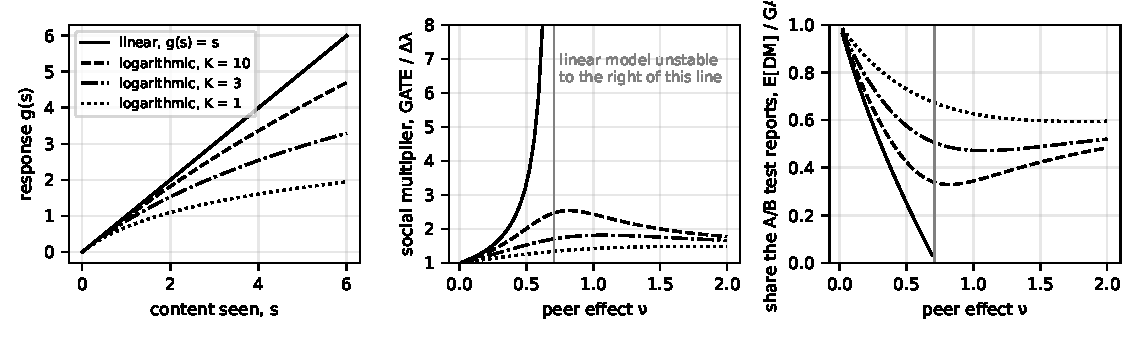
\includegraphics[width=\textwidth]{log_response.pdf}
\caption{Left: the linear response and the logarithmic response for three values of $K$.  Middle and right: the social multiplier GATE$/\Delta\lambda$ and the share of the launch effect that the A/B test reports, E[DM]$/$GATE, on the three-user graph against the peer effect $\nu$, with the line styles of the left panel; computed numerically by iteration.  The vertical line is $\nu = 1/\sqrt2$, where the linear model becomes unstable.}
\label{fig:log}
\end{figure}

\textbf{What changes with the peer effect.}  Figure~\ref{fig:log} repeats the computation for $\nu$ from 0 to 2.  In the linear model the multiplier diverges at $\nu = 1/\sqrt2$ and the A/B test sees almost nothing of the effect near that point.  With the logarithm the multiplier stays bounded, and it peaks and then falls ($K = 10$ at $\nu \approx 0.8$, $K = 3$ at $\nu \approx 1.1$, $K = 1$ at $\nu \approx 1.8$).  A stronger peer effect raises everybody's posting, and exposure, the sum of the friends' posting, grows faster than $\nu$; the slope $g'(s) = 1/(1 + s/K)$ then falls faster than $\nu$ grows, so each user's effective peer effect $\nu g'(s)$ in $\mathbf{J}$ shrinks.  The share the A/B test reports stays above 0.3, while in the linear model it falls to about 1.5\% at the stability limit on this graph.  The larger $K$, the longer the logarithmic model follows the linear one before it bends.

\section{Summary}

The quantities of this note, and what each of them means on any friendship graph:

\begin{itemize}
\item $\mA$, the friendship graph: $A_{ij} = 1$ if users $i$ and $j$ are friends.  Row $i$ of $\mA\vc(\vz)$ is what user $i$ sees from the friends.
\item $\mM = (\mI - \nu\mA)^{-1}$, the multiplier matrix: $M_{ij}$ is how much user $i$'s posting rises per extra post injected at user $j$, after all the back-and-forth through the friends has settled.  It is the sum over walks of all lengths from $i$ to $j$, each walk of length $k$ weighted by $\nu^k$.
\item $\rho(\mA)$, the spectral radius, and the stability condition $\nu\rho(\mA) < 1$: each round of feedback multiplies the extra posting by about $\nu\rho(\mA)$.  Below 1 the rounds shrink and the posting settles; at or above 1 they grow and posting runs away.  $\rho$ grows with hubs, so a few well-connected users can make a network unstable at a peer effect that is safe on average.
\item GATE $= \Delta\lambda\,\one^\top\mM\one/N$, the launch effect: the average extra posts per user if everybody gets the treatment.  It uses all of $\mM$, because every user's extra posting also reaches everybody else.
\item GATE$/\Delta\lambda$, the social multiplier: how much the treatment effect reinforces itself on the social graph.
\item ADE $= \Delta\lambda\,\mathrm{tr}(\mM)/N$, the average direct effect: the average extra posts of a user who is treated alone.  It uses only the diagonal of $\mM$, the part of a user's extra posting that comes back to that same user through the friends.
\item E[DM], what an A/B test reports on average: the ADE minus $(\text{GATE} - \text{ADE})/(N-1)$, so close to the ADE on a large graph whose multiplier is much smaller than $N$, not the GATE.  Treated and control users have on average the same share of treated friends, so they receive about the same spillover, the off-diagonal part of $\mM$, and the difference between the groups removes it; what remains is the $-(\text{GATE} - \text{ADE})/(N-1)$ term, which is small on a large graph.
\item With a logarithmic response the matrix formulas no longer apply and no closed form is known, but the steady state exists for every $\nu$ and is found by iteration; for small treatments the linear formulas hold approximately with $\mathbf{J} = \nu\,\mathrm{diag}(g'(\boldsymbol{s}))\mA$ in place of $\nu\mA$, which damps the users who see the most.
\item A single DM can even have the wrong sign, when users who post more for other reasons, such as the hub, land in the control group; over many assignments this averages out.
\end{itemize}

The same formulas hold on any graph, with $\mM$ computed numerically instead of by hand.  What changes on a large social network is the size of the terms: hubs make $\rho(\mA)$ large, and many friends per user make the off-diagonal part of $\mM$, the spillover, a large share of the launch effect.

{\scriptsize
\begin{thebibliography}{99}\setlength{\itemsep}{0pt}
\bibitem{aronow2017} P.~M. Aronow, C.~Samii. Estimating average causal effects under general interference, with application to a social network experiment. \emph{Annals of Applied Statistics} 11(4), 1912--1947, 2017.
\bibitem{ballester2006} C.~Ballester, A.~Calv\'o-Armengol, Y.~Zenou. Who's who in networks. Wanted: the key player. \emph{Econometrica} 74(5), 1403--1417, 2006.
\bibitem{belhaj2014} M.~Belhaj, Y.~Bramoull\'e, F.~Dero\"{\i}an. Network games under strategic complementarities. \emph{Games and Economic Behavior} 88, 310--319, 2014.
\bibitem{bonacich1987} P.~Bonacich. Power and centrality: a family of measures. \emph{American Journal of Sociology} 92(5), 1170--1182, 1987.
\bibitem{bramoulle2009} Y.~Bramoull\'e, H.~Djebbari, B.~Fortin. Identification of peer effects through social networks. \emph{Journal of Econometrics} 150(1), 41--55, 2009.
\bibitem{corless1996} R.~M. Corless, G.~H. Gonnet, D.~E.~G. Hare, D.~J. Jeffrey, D.~E. Knuth. On the Lambert W function. \emph{Advances in Computational Mathematics} 5(1), 329--359, 1996.
\bibitem{eckles2017} D.~Eckles, B.~Karrer, J.~Ugander. Design and analysis of experiments in networks: reducing bias from interference. \emph{Journal of Causal Inference} 5(1), 20150021, 2017.
\bibitem{horn2013} R.~A. Horn, C.~R. Johnson. \emph{Matrix Analysis}, 2nd edition. Cambridge University Press, 2013.
\bibitem{hudgens2008} M.~G. Hudgens, M.~E. Halloran. Toward causal inference with interference. \emph{Journal of the American Statistical Association} 103(482), 832--842, 2008.
\bibitem{katz1953} L.~Katz. A new status index derived from sociometric analysis. \emph{Psychometrika} 18(1), 39--43, 1953.
\bibitem{kennan2001} J.~Kennan. Uniqueness of positive fixed points for increasing concave functions on $\mathbb{R}^n$: an elementary result. \emph{Review of Economic Dynamics} 4(4), 893--899, 2001.
\bibitem{manski1993} C.~F. Manski. Identification of endogenous social effects: the reflection problem. \emph{Review of Economic Studies} 60(3), 531--542, 1993.
\bibitem{savje2021} F.~S\"avje, P.~M. Aronow, M.~G. Hudgens. Average treatment effects in the presence of unknown interference. \emph{Annals of Statistics} 49(2), 673--701, 2021.
\bibitem{ugander2013} J.~Ugander, B.~Karrer, L.~Backstrom, J.~Kleinberg. Graph cluster randomization: network exposure to multiple universes. \emph{KDD 2013}, 329--337, 2013.
\end{thebibliography}}

\end{document}
